\documentclass{beamer}
\usepackage[utf8]{inputenc}
\usepackage[T1]{fontenc}
\usepackage{graphicx}
\usepackage{appendixnumberbeamer}
\usepackage{booktabs}
\usepackage{bbm}
\usepackage[scale=2]{ccicons}
\usepackage{pgfplots}
\usepgfplotslibrary{dateplot}
\usepackage{xspace}
\newcommand{\themename}{\textbf{\textsc{metropolis}}\xspace}

\usetheme{metropolis}

\title{Rudarenje podataka LoRaWAN mreže}
%\subtitle{}
\date{\today}
\author{Ante Lojić Kapetanović}
\institute{FESB, Sveučilište u Splitu}

\begin{document}

  \maketitle

  \begin{frame}{Sadržaj}
    \setbeamertemplate{section in toc}[sections numbered]
    \tableofcontents[hideallsubsections]
  \end{frame}

  \section{Uvod i motivacija}
  \begin{frame}[fragile]{LoRaWAN - Long Range Wide Area Network}
    \alert{LoRaWAN} - dalekosežna mreža širokog područja definirana je kao protokol kontrole pristupa mediju (MAC) za mreže širokog područja (WAN).
    
    Dizajnirana je tako da zadovoljava ključna svojstva uređaja u IoT mreži:
    \begin{itemize}
      \item dalekosežno povezivanje
      \item skalabilnost
      \item energetska učinkovitost
    \end{itemize}
  \end{frame}
  
  \begin{frame}[fragile]
    \begin{center}
      \begin{figure}
        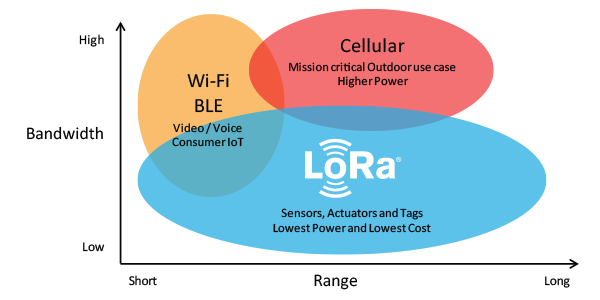
\includegraphics[width=\linewidth]{images/bw_range.png}
      \end{figure}
    \end{center}
  \end{frame}

  \begin{frame}{Arhitekturni pregled mreže}
    \begin{figure}
      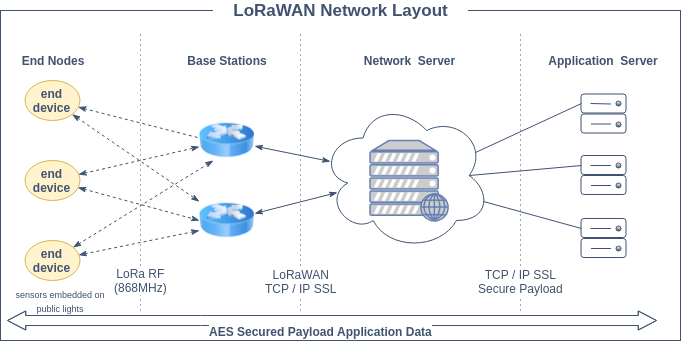
\includegraphics[width=\linewidth]{images/LoRaWAN-Network-Layout.png}
    \end{figure}
  \end{frame}

  \begin{frame}{Svebølle mrežna topologija}
    \begin{figure}
      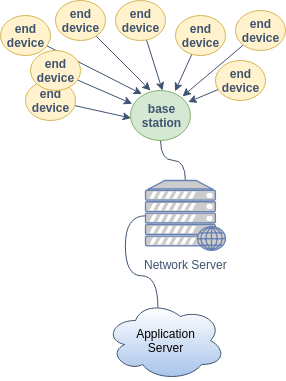
\includegraphics[width=0.48\linewidth]{images/Svebolle-Topology.png}
    \end{figure}
  \end{frame}

  \begin{frame}{Komunikacijski model za Svebølle implementaciju}
    \begin{figure}
      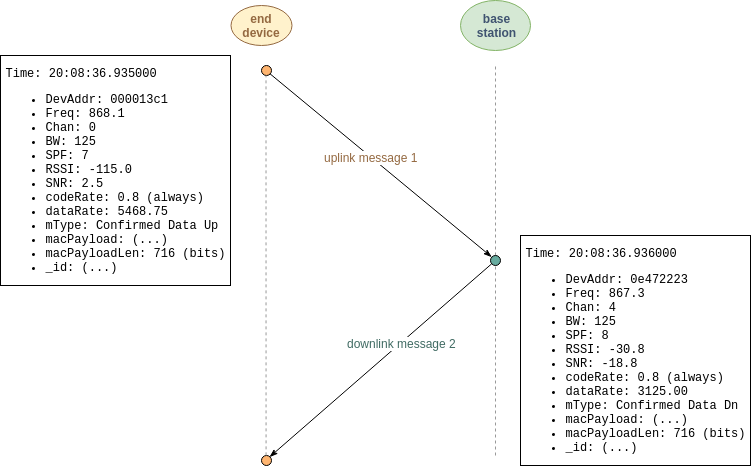
\includegraphics[width=\linewidth]{images/Svebolle-ed-bs-model.png}
    \end{figure}
  \end{frame}

  \begin{frame}{Cilj projekta}
    Je primjena prediktivnih statističkih metoda na mjerene podatke sa bazne stanice u Svebølleu i ispitivanje mogućnosti predviđanja \alert{uspješno transmitiranih LoRa poruka za dani interval vremena u budućnosti}.
  \end{frame}

  \begin{frame}{Motivacija}
    Uspješnom predikcijom aktivnosti krajnjih uređaja za blisku budućnost osigurao bi se prostor definiranju učinkovitijih pristupnih protokola što bi posljedično rezultiralo boljom mrežnom propusnošćuu i pouzdanošću same mreže ali i energetskom efikasnošću.
  \end{frame}

  \section{Prediktivne metode}
  \begin{frame}{Struktura mjerenih podataka}
    \begin{itemize}
      \item Podaci su prikupljeni kroz 5 mjeseci
      \item 689k mjerenja su snimljene na jednoj baznoj stanici
      \item Mjerene značajke\begin{itemize}
        \item Time
        \item DevAddr
        \item Freq, Chan, BW, CR, DR 
        \item RSSI, SNR  
        \item crcStatus, mType,macPayload 
      \end{itemize}
    \end{itemize}
  \end{frame}

  \begin{frame}{Transformacija snimljenih podataka u vremensku seriju}
    \alert{Vremenska serija} je niz sukcesivno raspoređenih elemenata indeksiranih u vremenskom redoslijedu pri čemu su elementi vremenski jednako razmaknuti.

    Kako bismo kreirali vremensku seriju, jedina bitna značajka podatkovnog seta je aktivnost uređaja u promatranom prošlom trenutku.
    Za svaki trenutak, gdje je trenutak u rezoluciji sekunde, zastavica aktivnosti je dodijeljenja na način:
    \begin{itemize}
      \item 1 - uređaj je bio aktivan u promatranom trenutak
      \item 0 - uređaj nije bio aktivan u promatranom trenutku
    \end{itemize}
  \end{frame}

  \begin{frame}{Prediktivni modeli}
    \begin{itemize}
      \item Moving average / weighted moving average
      \item Autoregressive integrated moving average (ARIMA)
      \item Holt's winter method
      \item Vector auto regression (VAR)
      \item \alert{Recurrent neural network (RNN)}
      \item Reinforcement learning (RL)
    \end{itemize}
  \end{frame}

  \section{Predloženi RNN model}
  \begin{frame}{Umjetna neuralna mreža}
    Prepoznaju regularnosti i uzorke promatranog seta podataka, uče iz prošlog iskustva i osiguravaju mogućnost zaključivanja na temelju izlaznih podataka.

    Jednostavne neuralne mreže nisu namjenjene za prognoziranje vremenskih serija jer su limitirane s mogućnošću pamćenja historijskih podataka.
  \end{frame}

  \begin{frame}{RNN mreža (Reccurent Neural Network)}
    \begin{columns}
      \column{.5\textwidth}
        RNN sadrži petlje (povratne veze) koje osiguravaju ustrajnost informacije.
      \column{.5\textwidth}
      \begin{figure}[]
        \centering
        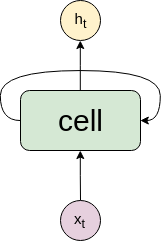
\includegraphics[width=0.6\linewidth]{images/RNN.png}
      \end{figure}
    \end{columns}
  \end{frame}
  \begin{frame}{Raspakirana RNN mreža}
    \begin{figure}[]
      \centering
      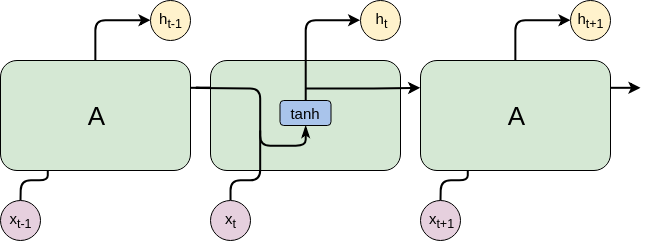
\includegraphics[width=\linewidth]{images/RNN-unpacked.png}
    \end{figure}
  \end{frame}
  \begin{frame}{Problem kratkoročne memorije}
    Ako je sekvenca podataka preduga, RNN mreža će imati problem pri prenošenju informacija iz historijskih momenata u kasnije momente.
    Razlog je jer tijekom povratne propagacije (\textit{back propagation}), RNN mreže pate od problema nestajućeg gradijenta (gradijent se smanjuje tijekom vremena povratne propagacije).

    \begin{center}
      \textbf{nova težina = težina - stopa učenja $\times$ gradijent}

      gradijent = 0 $\rightarrow$ nova težina = težina $\rightarrow$ RNN mreža prestaje učiti 
    \end{center}
  \end{frame}

  \begin{frame}{LSTM mreže (Long Short-Term Memory) u pomoć!}
    Promjena unutrašnje strukture RNN ćelije osigura se regulacija protočnosti informacije.

    Unutrašnjost svake LSTM ćelije je realizirana s mehanizmima zvanim \alert{vrata} koja kroz treniranje uče koji podaci sekvence su bitni a koji mogu biti odbačeni.
  \end{frame}
  \begin{frame}
    \begin{figure}[]
      \centering
      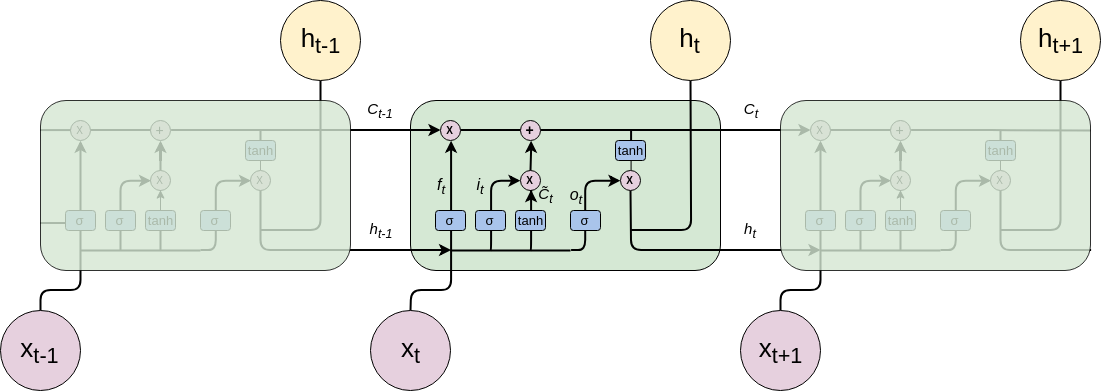
\includegraphics[width=\linewidth]{images/LSTM.png}
    \end{figure}
  \end{frame}

  \begin{frame}{'Forget' vrata}  
    određuju koju informaciju odbaciti iz \textit{stanja ćelije} koristeći sigmoidnu funkciju koja na izlazu daje rezultate između 0 (u potpunosti odbaciti) i 1 (u potpunosti prihvati)
    $$ f_{t} = \sigma (W_{f} \cdot [h_{t-1}, x_{t}] + b_{f}) $$
		gdje je
		\begin{itemize}
			\item[] $ x_{t} $ trenutni ulazni vektor podataka;
			\item[] $ h_{t-1} $ prethodna vrijednosti izlaza ćelije;
			\item[] $ W_{f} $ pridružena težinska vrijednost;
			\item[] $ b_{f} $ je dodani \textit{bias}.
    \end{itemize}
  \end{frame}

  \begin{frame}{Ulazna vrata}
    određuju koja nova informacija će biti upisana u \textit{stanje ćelije}.
    
    Prvo, sigmoidna funkcija odlučuje koju vrijednost ažurirati:
    $$ i_{t} = \sigma (W_{i} \cdot [h_{t-1}, x_{t}] + b_{i}) $$ 
    gdje je
    \begin{itemize}
      \item[] $ x_{t} $ trenutni ulazni vektor podataka;
      \item[] $ h_{t-1} $ prethodna vrijednosti izlaza ćelije;
      \item[] $ W_{i} $ pridružena težinska vrijednost;
      \item[] $ b_{i} $ je dodani \textit{bias}.
    \end{itemize}
  \end{frame}

  \begin{frame}{Stanje ćelije}
    ...nakon toga, \textit{tanh} sloj kreira vektor kandidata za trenutno stanje ćelije:
    $$ \tilde{C}_{t} = tanh (W_{C} \cdot [h_{t-1}, x_{t}] + b_{C}) $$
    gdje je
    \begin{itemize}
      \item[] $ x_{t} $ trenutni ulazni vektor podataka;
      \item[] $ h_{t-1} $ prethodna vrijednosti izlaza ćelije;
      \item[] $ W_{C} $ pridružena težinska vrijednost;
      \item[] $ b_{C} $ je dodani \textit{bias}.
    \end{itemize}
  \end{frame}

  \begin{frame}{Izlazna vrata}
    određuju što ide na izlaz promatrane ćelije.
    $$ o_{t} = \sigma (W_{o} [h_{t-1}, x_{t}] + b_{o}) $$ 
    where
    \begin{itemize}
      \item[] $ x_{t} $ trenutni ulazni vektor podataka;
      \item[] $ h_{t-1} $ prethodna vrijednosti izlaza ćelije;
      \item[] $ W_{o} $ pridružena težinska vrijednost;
      \item[] $ b_{o} $ je dodani \textit{bias}.
    \end{itemize}
    
    Izlaz je baziran na filtriranoj verziji \textit{stanja ćelije}.
    $$ h_{t} = o_{t} * tanh(C_{t})$$
    gdje je 
    $ C_{t} $ novo stanje dobiveno kroz:
    $ C_{t} = f_{t} * C_{t-1} + i_{t} * \tilde{C}_{t} $
  \end{frame}

  \section{Rezultati}
  \begin{frame}{Predprocesiranje}
    \begin{enumerate}
      \item čišćenje
      \item čisti podatkovni set $\rightarrow$ vremenska serija
      \item kreiranje sekvenca
      \item randomiziranje sekvenca 
      \item podjela podatkovnog seta na set za trening i set za validaciju rezultata
    \end{enumerate}
  \end{frame}

  \begin{frame}{Validacijski rezultati}
    \begin{figure}[]
      \centering
      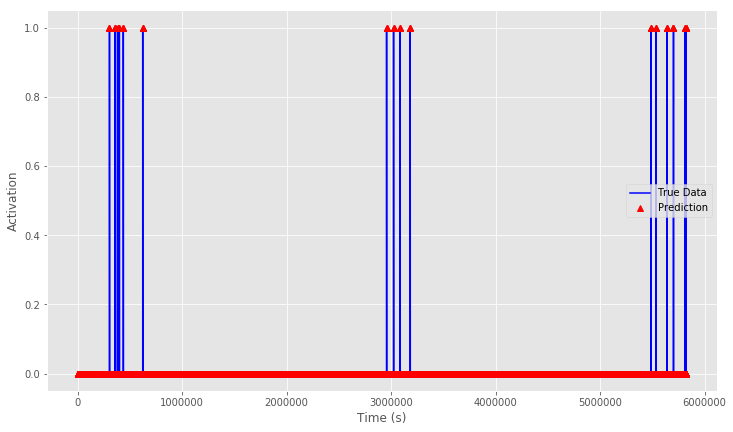
\includegraphics[width=\linewidth]{images/lstm-out.png}
    \end{figure}
  \end{frame}

  \begin{frame}{Pogreške}
    \begin{figure}[]
      \centering
      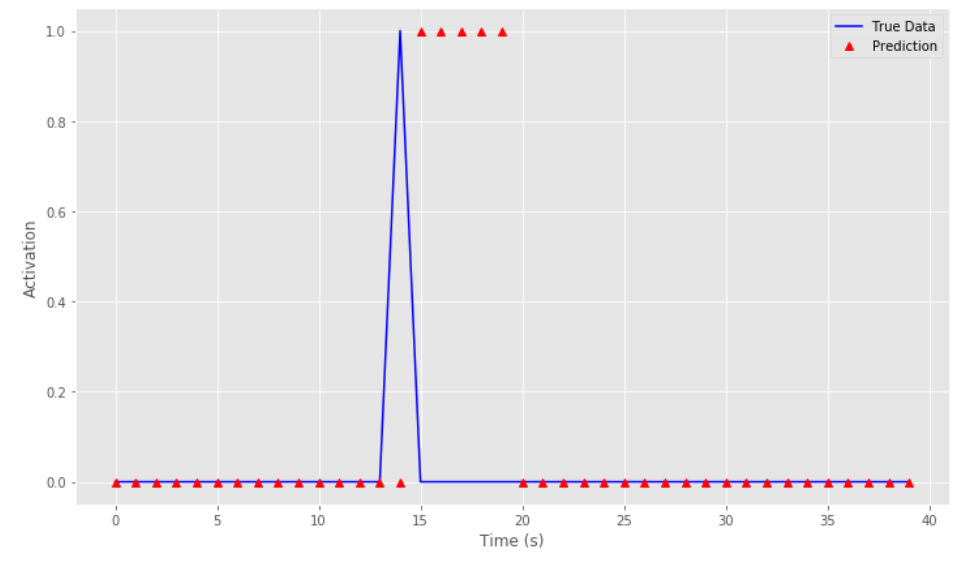
\includegraphics[width=\linewidth]{images/err.png}
    \end{figure}
  \end{frame}

  \begin{frame}{Validacija rezultata}
    \begin{figure}[]
      \centering
      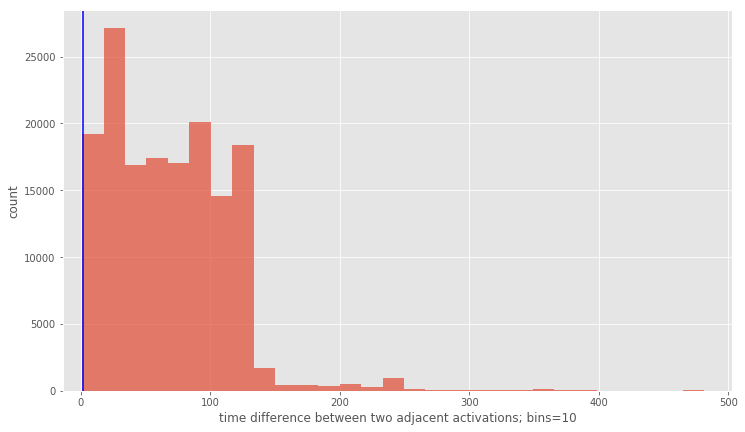
\includegraphics[width=\linewidth]{images/err_con.png}
    \end{figure}
    Za MAE=2s, 0.35\% pogrešnih predikcija.
  \end{frame}

  \begin{frame}{Procjena vjerojatnosti transmisije za proizvoljni budući vremenski period}
    Za dani vremenski period (\textbf{n} sekunda) vjerojatnost uspješne transmisije LoRa poruke s krajnjeg uređaja na baznu stanicu bi trebala rasti kako se povećava vremenski period (\textbf{n} postaje veći). 
    $$ n = 0 \Rightarrow p_{st} = 0 $$ 
    $$ n \in <0, +\infty> \Rightarrow p_{st} \in <0, 1> $$
    $$ n = \infty \Rightarrow p_{st} = 1 $$

    \end{frame}

  \begin{frame}
    \begin{figure}[]
      \centering
      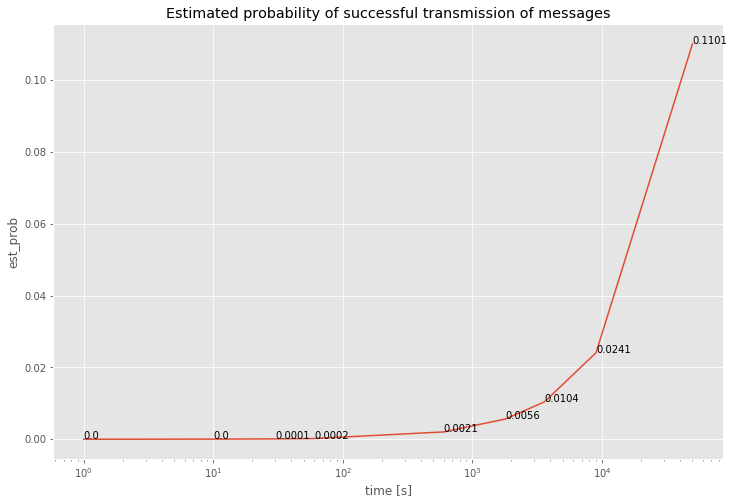
\includegraphics[width=\linewidth]{images/est-prob.png}
    \end{figure}
  \end{frame}


  \section{Zaključak}
  \begin{frame}{Budući rad}
    \begin{itemize}
      \item \textbf{Multivarijatna vremenska serija} umjesto jednostavne vremenske serije: promatrati ne samo prethodne historijske događaje za specifični uređaj nego i za ostale uređaje
      \item \textbf{Veće sekvence za treniranje modela}
      \item \textbf{Sekvencne predikcije} umjesto od-točke-do-toče predikcije
    \end{itemize}
  \end{frame}

  \begin{frame}[standout]
    Pitanja
  \end{frame}

  
\end{document}